\subsection{B$\acute{e}$zier Curves(贝赛尔曲线)}



\frame{
Pierre B$\acute{e}$zier at Renault\footnote{雷诺} and Paul de Casteljau\footnote{卡斯特利乌} at Citro$\textdoublevbaraccent{e}$n\footnote{雪铁龙} independently developed the {\Large B$\acute{e}$zier curve} for CAD/CAM operations, in the 1970s. 
\begin{itemize}
\item These parametrically defined polynomials are a class of approximating splines. 
\item B$\acute{e}$zier curves are the basis of the entire Adobe PostScript drawing model that is used in the software products Adobe Illustrator, Macromedia Freehand, and Fontographer. 
\item B$\acute{e}$zier curves continue to be the primary method of representing curves and surfaces in computer graphics (CAD/CAM\footnote{computer-aided geometric design}). 
\end{itemize}
}

\frame{
In Casteljau's original development, B$\acute{e}$zier curves were defined implicitly by a recursive algorithm (see Property 1 below). \\
\vspace{2cm}
The development of the properties of B$\acute{e}$zier curves will be facilitated by defining them explicitly in terms of {\Large Bernstein polynomials}. 
}

\frame{
\begin{block}{Definition 4.2.}
{\Large Bernstein polynomials} of degree $N$ are defined by
\begin{equation*}
B_{i,N} (t) = \left( \begin{array}{c} N \\ i \end{array} \right)
t^i (1-t)^{N-i}
\end{equation*}
for $i=0, 1, 2, \ldots, N$, where 
\begin{equation*}
\left( \begin{array}{c} N \\ i \end{array} \right) = \frac{N!}{i! (N-i)!}
\end{equation*} 
\end{block}
%\begin{figure}
%\begin{center}
%\includegraphics[width=110mm]{fig/ch-4/def_4-2.png}
%\end{center}
%\end{figure}
In general, there are $N + 1$ Bernstein polynomials of degree $N$. 
For example, the Bernstein polynomials of degrees $1$, $2$, and $3$ are
\begin{equation*}
B_{0,1} ( t ) = 1-t, \ \ B_{1,1} (t) = t
\end{equation*}
\begin{equation*}
B_{0,2}(t) = (1-t)^2, \ \ B_{1,2}(t) = 2t (1-t), \ \ B_{2,2} (t) = t^2
\end{equation*}
\begin{equation*}
B_{0,3} (t) = (1-t)^3, \ \ B_{1,3} (t) = 3t (1-t)^2, \ \  B_{2,3}(t) = 3t^2(1-t), \ \ B_{3,3}(t) = t^3
\end{equation*}
%\begin{figure}
%\begin{center}
%\includegraphics[width=110mm]{fig/ch-4/def_4-2_2.png}
%\end{center}
%\end{figure}
}

\frame{
\frametitle{Properties of Bernstein Polynomials}
\begin{block}{Property 1. Recurrence Relation}
Bernstein polynomials can be generated in the following way. 
Set $B_{0,0} (t) = 1$ and $B_{i,N} (t) = 0$ for $i < 0$ or $i > N$, and use the recurrence relation
\begin{equation*}
B_{i,N} (t) = (1 - t) B_{i, N-1} (t) + t B_{i-1,N-1}(t) 
\end{equation*}
for $i = 1$, $2$, $3$, $\ldots$, $N - 1$.
\end{block}
\begin{columns}
\begin{column}{0.6\textwidth}
\begin{block}{Property 2. Nonnegative on $[0, 1]$}
The Bernstein polynomials are nonnegative over the interval $[0, 1]$
\end{block}
\end{column}
\begin{column}{0.4\textwidth}
\begin{figure}
\begin{center}
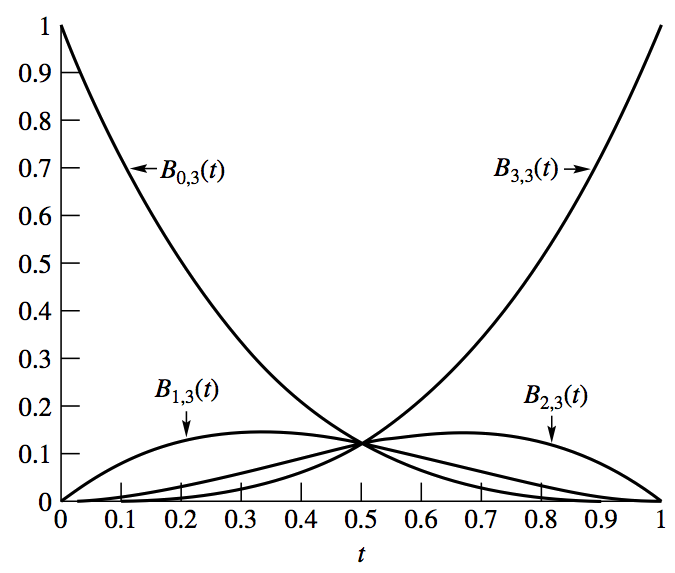
\includegraphics[width=40mm]{chap-4/fig_5-21.png}
\end{center}
\end{figure}
\end{column}
\end{columns}
}

\frame{
\begin{block}{Property 3.} 
The Bernstein polynomials form a partition of unity
\begin{equation*}
\sum_{i=0}^N B_{i,N} (t) = 1
\end{equation*}
Substituting $x = t$ and $y = 1 - t$ into the binomial theorem
\begin{equation*}
(x + y)^N = \sum_{i=0}^N
\left( \begin{array}{c}
N \\
i 
\end{array} \right)
x^i y^{N-i}
\end{equation*}
yields
\begin{equation*}
\sum_{i=0}^N
\left( \begin{array}{c}
N \\
i 
\end{array} \right)
x^i y^{N-i} = (t + (1 - t))^N = 1^N = 1.
\end{equation*}
\end{block}
}

\frame{
\begin{block}{Property 4. Derivatives}
\begin{equation*}
\frac{d}{d t} B_{i,N} (t) =N \left( B_{i-1,N-1} (t) - B_{i,N-1}(t) \right)
\end{equation*}
Formula (4.80) is established by taking the derivative of the Bernstein polynomial in Definition 4.2.
\begin{equation*}
\begin{array}{l c l}
\frac{d}{d t} B_{i,N} (t) & = & \frac{d}{dt} \left( \begin{array}{c} N \\ i  \end{array} \right)  t^i (1-t)^{N-i} \\
 & = & \frac{i N!}{i ! (N-i)!} t^{i-1}(1-t)^{N-i} - \frac{(N-i)N!}{i! (N-i)!} t^i (1-t)^{N-i-1} \\
 & = & \frac{ N (N-1)!}{(i-1)! (N-i)!} t^{i-1}(1-t)^{N-i} - \frac{N(N-1)!}{i! (N-i+1)!} t^i (1-t)^{N-i-1}  \\
 & = & N \left( \frac{(N-1)!}{(i-1)! (N-i )!} t^{i-1}(1-t)^{N-i} - \frac{(N-1)!}{i ! (N-i-1)!} t^i (1- t)^{N-i-1} \right) \\
& = & N \left( B_{i-1,N-1} (t) - B_{i,N-1} (t) \right)
\end{array}
\end{equation*}
\end{block}
}

\frame{
\begin{block}{Property 5. Basis}
The Bernstein polynomials of order $N(B_{i,N}(t))$ for $i = 0$, $1$, $\ldots$, $N$ form a basis of the space of all polynomials of degree less than or equal to $N$.
\end{block}
Property 5 states than any polynomial of degree less than or equal to $N$ can be written uniquely as a linear combination of the Bernstein polynomials\footnote{伯思斯坦多项式} of order $N$. \\ 
%The concept of a basis of a vector space is introduced in Chapter 11.
Given a set of control points, $\{ P_i \}^N_{i=0}$, a B$\acute{e}$zier curve of degree $N$ is now defined as a weighted sum of the Bernstein polynomials of degree $N$.
}

\frame{
\begin{block}{Definition 4.3.} 
Given a set of control points $\{ P_i \}^N_{i=0}$, where $P_i = (x_i, y_i )$, a B$\acute{e}$zier curve of degree $N$ is
\begin{equation*}
P(t) = \sum_{i=0}^N P_i B_{i, N}(t)
\end{equation*}
where $B_{i,N} (t)$, for $i = 0$, $1$, $\ldots$, $N$, are the Bernstein polynomials of degree $N$, and $t \in [0, 1]$.
\end{block}
In formula (4.81) the control points are ordered pairs representing $x-$ and $y-$coordinates in the plane.  \\
Without ambiguity the control points can be treated as vectors and the corresponding Bernstein polynomials as scalars. 
}

\frame{
Thus formula (4.81) can be represented parametrically as $P(t) = (x(t), y(t))$, where 
\begin{equation*}
x(t) = \sum_{i=0}^N x_i B_{i, N}(t) \ \ \ and \ \ \ y(t) = \sum_{i=0}^N y_i B_{i, N}(t)
\end{equation*}
and $0 \le t \le 1$. 
The function $P(t)$ is said to be a vector-valued function, or equivalently, the range of the function is a set of points in the $xy-$plane. 
}

\frame{
\frametitle{Example 4.13.} 
Find the B$\acute{e}$zier curve which has the control points $(2, 2)$, $(1, 1.5)$, $(3.5, 0)$, and $(4, 1)$.

Substituting the $x-$ and $y-$ coordinates of the control points and $N = 3$ into formula (4.82) yields
\begin{equation*}
x(t) = 2 B_{0,3}(t) + 1 B_{1,3}(t) + 3.5 B_{2,3}(t) + 4 B_{3,3}(t)
\end{equation*}
\begin{equation*}
y(t) = 2 B_{0,3}(t) + 1.5 B_{1,3}(t) + 0 B_{2,3}(t) + 1 B_{3,3}(t).
\end{equation*}
Substituting the Bernstein polynomials of degree three, found in formula (4.77), into formulas (4.83) and(4.84) yields
\begin{equation*}
x(t) = 2 (1 - t)^3 + 3 t (1 - t)^2 + 10.5 t^2 (1 - t) + 4 t^3
\end{equation*}
\begin{equation*}
y(t) = 2 (1 - t)^3 + 4.5 t (1 - t)^2 + t^3.
\end{equation*}
}

\frame{
Simplifying formulas (4.85) and (4.86) yields
\begin{equation*}
P(t) = \left( 2 - 3t + 10.5t^2 - 5.5t^3,   2 - 1.5t - 3t^2 + 3.5t^3 \right),
\end{equation*}
where $0 \le t \le 1$.
\begin{figure}
\begin{center}
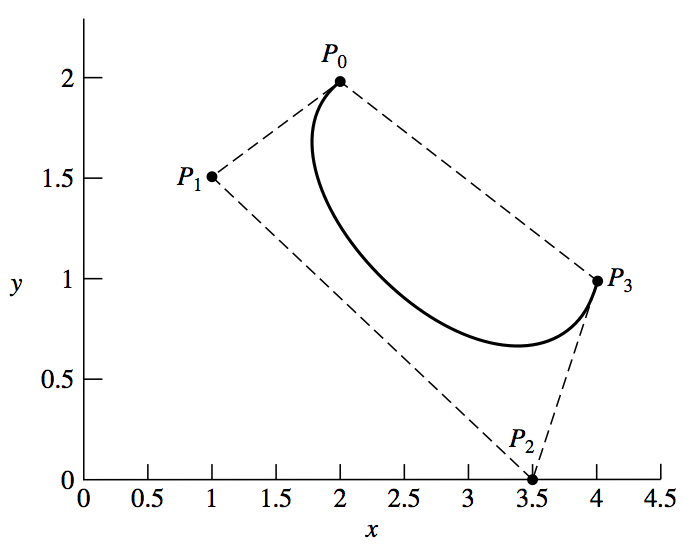
\includegraphics[width=70mm]{chap-4/fig_5-22.png}
\end{center}
\end{figure}
}


\frame{
\begin{itemize}
\item The functions $x(t)$ and $y(t)$ in formulas (4.85) and (4.86) are polynomials and are continuous and differentiable over the interval $0 \le t \le 1$. 
\item Thus the graph of the Bezier curve $P(t)$ is a continuous and differentiable curve in the $xy-$plane (see Figure 4.18), where $0 \le t \le 1$. 
\item Note. $P(0) = (2,2)$ and $P(1) = (4,1)$. 
\item The graph of the curve starts at the first control point $(2,2)$ and ends at the last control point $(4,1)$. 
\end{itemize}
}


\frame{
\frametitle{Properties of B$\acute{e}$zier Curves}
\begin{block}{Property 1. The points $P_0$ and $P_1$ are on the curve $P(t)$}
Substituting $t = 0$ into Definition 4.2 yields
\begin{equation*}
B_{i,N} (0) = \left\{  
\begin{array}{l l l}
1 & for & i = 0 \\
0 & for & i \neq 0 
\end{array}
\right.
\end{equation*}
Similarly, $B_{i,N}(1) = 1$ for $i = N$ and is zero for $i = 0, 1, \ldots, N - 1$. 
Substituting these results into Definition 4.3 yields
\begin{equation*}
P(0) = \sum_{i=0}^N P_i B_{i,N}(0) = P_0
\ \ \ and \ \ \ 
P(1) = \sum_{i=0}^N P_i B_{i,N}(1) = P_N
\end{equation*}
\end{block}
Thus the first and last points in the sequence of control points, $\{ P_i \}^N_{i=0}$, are the endpoints of the B$\acute{e}$zier curve. 
%Note. The remaining control points are not necessarily on the curve.
%\begin{figure}
%\begin{center}
%\includegraphics[width=110mm]{fig/ch-4/p_195-1.png}
%\end{center}
%\end{figure}
}

\frame{
\begin{itemize}
\item In Example 4.13 there were four control points and the resulting components $x(t)$ and $y(t)$ were third-degree polynomials. 
\item In general, when there are $N + 1$ control points the resulting components will be polynomials of degree $N$. 
\item Since polynomials are continuous and have continuous derivatives of all orders, it follows that the B$\acute{e}$zier curve in Definition 4.3 will be continuous and have derivatives of all orders. 
\end{itemize}
}

\frame{
\begin{block}{Property 2. $P(t)$ is continuous and has derivatives of all orders on the interval $[0, 1]$}
The derivative of $P(t)$, with respect to $t$, is
\begin{equation*}
\begin{array}{l c l}
P'(t) & = & \frac{d}{dt} \sum_{i=0}^N P_i B_{i,N} (t) \\
 & = & \sum_{i=0}^N P_i \frac{d}{dt} B_{i,N} (t) \\
 & = & \sum_{i=0}^N P_i N \left( B_{i-1, N-1} (t) - B_{i, N-1} (t) \right)
\end{array}
\end{equation*}
\end{block}
(Property 4 of Bernstein polynomials). 
Setting $t = 0$ and substituting $B_{i,N} (0) = 1$ for $i = 0$ and $B_{i,N} (0) = 0$ for $i \ge 1$\footnote{(Definition 4.2)} into the right-hand side of the expression for $P'(t)$ and  simplifying yields
\begin{equation*}
P'(0) = \sum^N_{i=0} P_i N \left( B_{i-1, N-1}(0) - B_{i,N-1}(0) \right) = N(P_1 - P_0)
\end{equation*}
}

\frame{
Similarly, $P'(1) = N(P_N - P_{N-1})$. 
In other words, the tangent lines to a B$\acute{e}$zier curve at the endpoints are parallel to the lines through the endpoints and the adjacent control points. 
The property is illustrated in Figure 4.19. 
\begin{figure}
\begin{center}
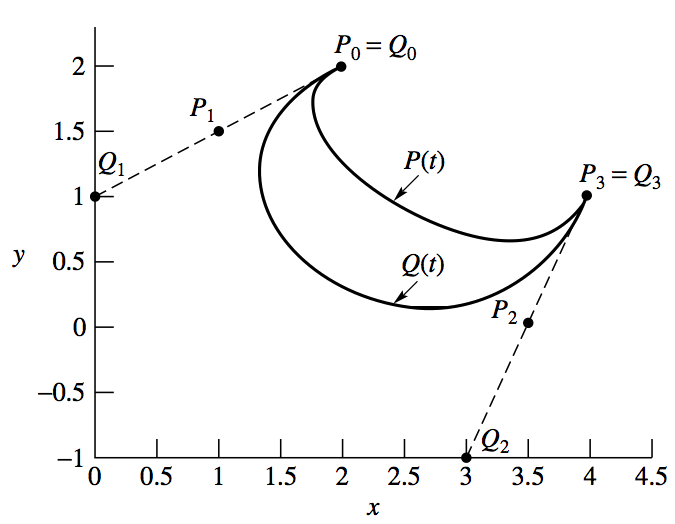
\includegraphics[width=50mm]{chap-4/fig_5-23.png}
\end{center}
\end{figure}
}

\frame{
\begin{block}{Property 3. $P'(0)=N(P_1 - P_0)$ and $P'(1)=N(P_N - P_{N-1})$} 
\begin{itemize}
\item The final property is based on the concept of a {\Large convex set}. 
\item $A$ subset $C$ of the $xy-$plane is said to be a convex set, provided that all the points on the line segment joining any two points in $C$ are also elements of the set $C$. 
\item For example, a line segment or a circle and its interior are convex sets, while a circle without its interior is not a convex set. 
\item The convex set concept extends naturally to higher-dimension spaces. 
\end{itemize}
\end{block}
}


\frame{
\begin{block}{Definition 4.4.} 
The {\Large convex hull} of a set $C$ is the intersection of all convex sets containing $C$.
\end{block}
Figure 4.18 shows the convex hull (the indicated quadrilateral and its interior) of the control points for the B$\acute{e}$zier curve from Example 4.13. 
In the $xy-$plane the convex hull of a set of points, $\{ P_i \}^N_{i=0}$, may be visualized by placing pins at each point and placing a rubber band around the resulting configuration.
}

\frame{
A sum $\sum^N_{i=0} m_i P_i$ is said to be a convex combination of the points $\{ P_i \}^N_{i=0}$, provided that the set of coefficients $m_0$, $m_1$, $\ldots$, $m_N$ are nonnegative and $\sum^N_{i=0} m_i = 1$.
A convex combination of points must necessarily be a subset of the convex hull of the set of points. 
It follows from properties 2 and 3 of the Bernstein polynomials that the B$\acute{e}$zier curve in formula (4.81) is a convex combination of the control points. 
Therefore, the graph of the curve must lie in the convex hull of the control points.
}


\frame{
\begin{block}{Property 4.}
 The B$\acute{e}$zier curve lies in the convex hull of its set of control points
\end{block}
%\begin{figure}
%\begin{center}
%\includegraphics[width=110mm]{fig/ch-4/p_196-1.png}
%\end{center}
%\end{figure}
\begin{itemize}
\item The properties indicate that the graph of a Bezier curve of degree $N$ is a continuous curve, bounded by the convex hull of the set of control points, $\{ P_i \}^N_{i=0}$, and that the curve begins and ends at points $P_0$ and $P_N$, respectively. 
\item B$\acute{e}$zier observed that the graph is sequentially pulled toward each of the remaining control points $P_1, P_2, \ldots ,P_{N-l}$·
\end{itemize}
}

\frame{ 
\begin{itemize}
\item For example, if the control points $P_1$ and $P_{N-1}$ are replaced by the control points $Q_1$ and $Q_{N-1}$ which are farther away (but in the same direction) from the respective endpoints, then the resulting B$\acute{e}$zier curve will more closely approximate the tangent line near the endpoints. 
\item Figure 4.19 illustrates the pulling and tangent effects using the B$\acute{e}$zier curve $P(t)$ from Example 4.16 and the curve $Q(t)$ with control points $(2,2)$, $(0, 1)$, $(3, -1)$, and $(4,1)$. Clearly, $Q_1$, $P_1$, and $P_0 = Q_0$, and $Q_2$, $P_2$, and $P_3 = Q_3$ are collinear, respectively. 
\end{itemize}
}

\frame{
\begin{itemize}
\item The effectiveness of B$\acute{e}$zier curves lies in the ease with which the shape of the curve can be modified (mouse, keyboard, or other graphical interface) by making small adjustments to the control points. 
\item Figure 4.20 shows four B$\acute{e}$zier curves, of different degrees, with the corresponding sets of control points sequentially connected to form polygonal paths. 
\item The reader should observe that the polygonal paths provide a rough sketch of the resulting B$\acute{e}$zier curves. 
Changing the coordinates of anyone control point, say $P_k$, will change the shape of the entire curve over the parameter interval $0 \le t \le 1$. 
\end{itemize}
}

\frame{
\begin{itemize}
\item The changes in the shape of the curve will be somewhat localized, since the Bernstein polynomial $B_{k,N}$, corresponding to the control point $P_k$ (formula (4.81)) , has a maximum at the parameter value $t = k / N$. 
\item Thus the majority of the change in the shape ofthe graph of the B$\acute{e}$zier curve will occur near the point $P (k / N)$. 
\item Consequently, creating a curve of a specified shaped requires a relatively small number of changes to the original set of control points. 
\end{itemize}
}


\frame{
\begin{figure}
\begin{center}
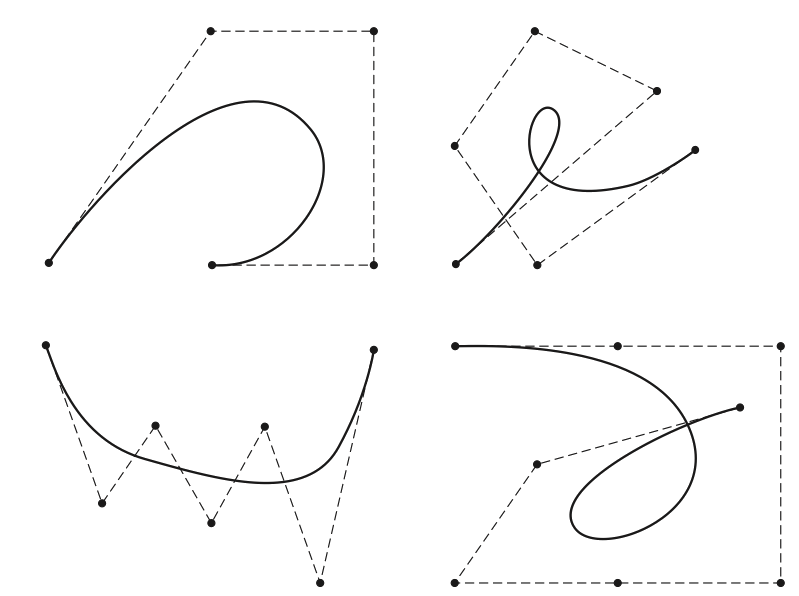
\includegraphics[width=80mm]{chap-4/fig_5-24.png}
\end{center}
\end{figure}
}

\frame{
\begin{itemize}
\item In practice, curves are produced using a sequence of B$\acute{e}$zier curves sharing common endpoints. 
\item This process is analogous to that used in the creation of cubic splines. 
\item In that case it was necessary to use a sequence of cubic polynomials to avoid the oscillatory behavior of polynomials of high degree. 
\item Property 4 shows that the oscillatory behavior of higher-degree polynomials is not a problem with B$\acute{e}$zier curves. 
\item Since changing one control point changes the shape of a B$\acute{e}$zier curve, it is simpler to break the process into a series of B$\acute{e}$zier curves and minimize the number of changes in the control points. 
\end{itemize}
}



\frame{
\frametitle{Example 4.14.} 
Find the composite B$\acute{e}$zier curve for the four sets of control points
\begin{equation*}
\begin{array}{c c}
\left\{ (-9, 0), (-8, 1), (-8, 2.5), (-4, 2.5) \right\}, & \left\{ (-4, 2.5), (-3, 3.5), (-1, 4), (0, 4) \right\} \\
\left\{ (0, 4), (2, 4), (3, 4), (5, 2) \right\}, & \left\{ (5, 2), (6, 2), (20, 3), (18, 0) \right\}
\end{array}
\end{equation*}
Following the process outlined in Example 5.16 yields
\begin{equation*}
\begin{array}{l c l}
P_1(t) & = & (-9 + 3t - 3t^2 + 5t^3, 3t + 1.5t^2 - 2t^3) \\
P_2(t) & = & (-4 + 3t + 3t^2 - 2t^3, 2.5 + 3t - 1.5t^2) \\
P_3(t) & = & (6t - 3t^2 + 2t^3, 4 - 2t^3) \\
P_4(t) & = & (5 + 3t + 39t^2 - 29t^3, 2 + 3t^2 - 5t^3).
\end{array}
\end{equation*}
}

\frame{
The graph of the composite B$\acute{e}$zier curve and corresponding control points is shown in Figure 4.21.
\begin{figure}
\begin{center}
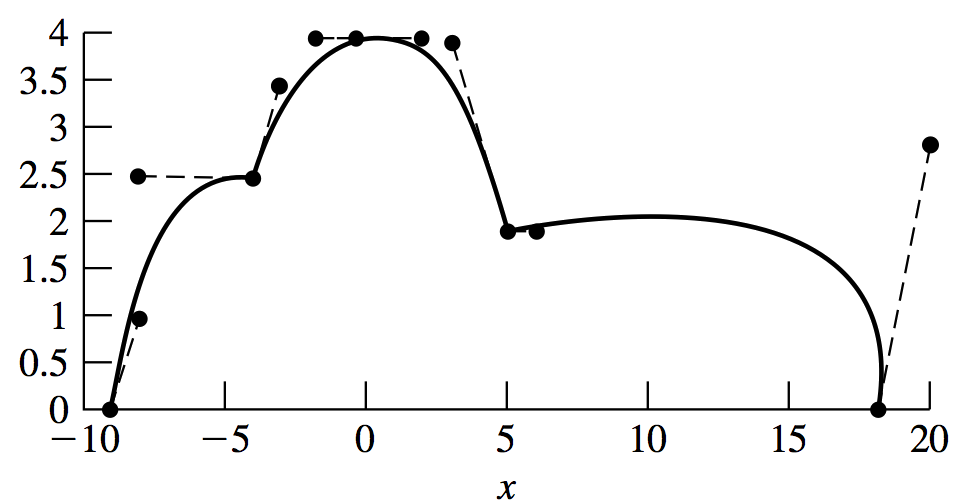
\includegraphics[width=80mm]{chap-4/fig_5-25.png}
\end{center}
\end{figure}
}


\frame{
\begin{itemize}
\item The B$\acute{e}$zier curves in Example 4.14 do not meet {\Large smoothly} at the common endpoints. 
\item To have two B$\acute{e}$zier curves $P(t)$ and $Q(t)$ meet smoothly would require that $P_N = Q_0$ and $P'(P_N) = Q'(Q_0)$. 
\item Property 3 indicates that it is sufficient to require that the control points $P_{N -1}, P_N = Q_0$, and $Q_1$ be collinear. 
\item To illustrate, consider the B$\acute{e}$zier curves $P(t)$ and $Q(t)$ of degree three with the control point sets 
\begin{equation*}
\left\{ (0, 3), (1, 5), (2, 1), (3, 3) \right\}
\end{equation*}
and
\begin{equation*}
\left\{ (3, 3), (4, 5), (5, 1), (6, 3) \right\},
\end{equation*}
respectively. 
\end{itemize}
}

{\frame{
Clearly, the control points $(2,1)$, $(3,3)$, and $(4,5)$ are collinear. 
Again, following the process outlined in Example 4.13: 
\begin{equation*}
P(t) = \left( 3^t, 3 + 6t - 18t^2 + 12t^3 \right)
\end{equation*}
\begin{equation*}
Q(t) = \left( 3 + 3t, 3 + 6t - 18t^2 + 12t^3 \right)
\end{equation*}
%\begin{figure}
%\begin{center}
%\includegraphics[width=80mm]{fig/ch-4/eq_4-87_2.png}
%\end{center}
%\end{figure}
and 
\begin{equation*}
P'(t) = \left( 3, 6 - 36t + 36t^2 \right)
\ \ \ and \ \ \ 
Q'(t) = \left( 3, 6 - 36t + 36t^2 \right)
\end{equation*}

%\begin{figure}
%\begin{center}
%\includegraphics[width=80mm]{fig/ch-4/eq_4-87_3.png}
%\end{center}
%\end{figure}
Substituting $t = 1$ and $t = 0$ into $P'(t)$ and $Q'(t)$, respectively, yields 
\begin{equation*}
P'(1) = (3, 6) = Q'(0)
\end{equation*}

%\begin{figure}
%\begin{center}
%\includegraphics[width=40mm]{fig/ch-4/eq_4-87_4.png}
%\end{center}
%\end{figure}
}

\frame{
The graphs of $P(t)$ and $Q(t)$ and the smoothness at the common endpoint are shown in Figure 4.22. 
\begin{figure}
\begin{center}
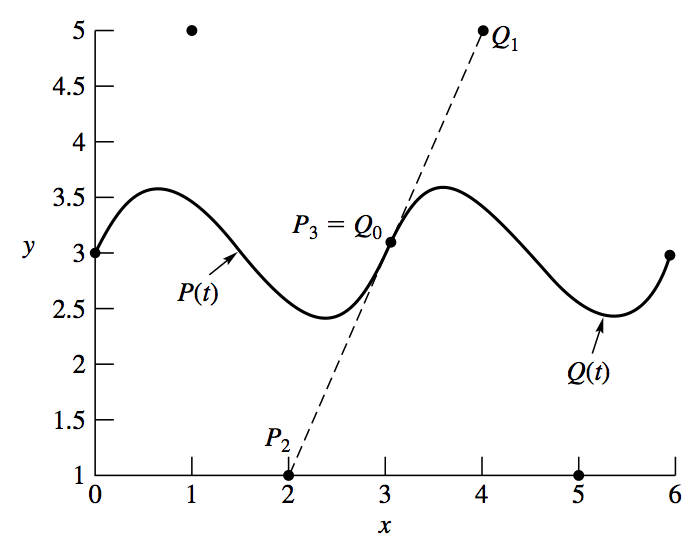
\includegraphics[width=80mm]{chap-4/fig_5-26.png}
\end{center}
\end{figure}
}

%\frame{
%The plot command is used to graph parametric curves in MATLAB. 
%The B$\acute{e}$zier curve in Example 4.13 can be plotted as follows: 
%\begin{figure}
%\begin{center}
%\includegraphics[width=60mm]{fig/ch-4/p_199-1.png}
%\end{center}
%\end{figure}
%}
